\chapter{设计结果}\label{chap:design}
由于双发射乱序处理器的结构复杂,细节众多,不可能事无巨细交代清楚。所以在本章节中,强调在设计过程中不同考虑的分析取舍和突出微结构设计中的亮点。
\section{处理器框架}
这里的框架指的是一种比微结构更加抽象的解耦合模型 --- 前端(Frontend)、后端(Backend)模型。在章节\ref{subsec:BOOM}中分析BOOM时已经做过了初步的介绍。
\begin{enumerate}[label=(\alph*)]
	\item 前端: 提供稳定的指令流,具体来说就是从初始地址开始源源不断地取回指令提供给后端处理。
	\item 后端: 接受来自前端的指令,进行运算,最后写回寄存器堆或内存。
\end{enumerate}
这个模型的优势在归纳起来:
\begin{enumerate}[label=(\alph*)]
	\item 前端不需要关心后端指令执行的机制;后端也不需要在乎前端取指状态机的运转流程以及所采用的缓存策略。例如对于可被缓存区域的取指,可以利用cache提高取指效率,也可以不用。
	\item 连接两端之间接口的信号非常少而且清晰。屈指可数 --- 前端到后端方向有指令以及指令是否有效,指令所在的PC,以及下一条PC的转移猜测信息;后端向前端有对于指令流的反馈如取回的指令是不是由于流水线的繁忙而需要阻塞,分支跳转类指令和例外中断对于指令流的重定向信息,以及对于转移预测数据结构的反馈更新。
	\item 前后端的解耦合模型,清晰的接口对于功能的调试、性能的调优也大有助益。
\end{enumerate}
%However, the kill signal is delayed a cycle for critical path reasons. BOOM的做法和我的类似
%BOOM (currently) does not rename any of the CSRs, and in addition to the potential side-effects caused by reading or writing a CSR, BOOM will only execute a CSR instruction non-speculatively. 
\section{处理器高性能因素考量}
衡量高性能的通用处理器有两个维度:频率(时钟一周期经过的时间)和IPC(单位周期完成的指令数)。不同于IPC维度是硬指标,频率这个维度,不同的硬件实现(FPGA/ASIC),同一逻辑的不同写法,甚至不同的综合工具都会对其有较大的影响,一个比较客观的分析方法是计算从一个触发器的Q端到下一个触发器的D端之间最多的门级数(在设计的时候靠着经验进行大致的估算和衡量,但是由于扇入扇出的影响,会存在误差)。因为现阶段刚刚完成了处理器的设计,还未来得及在综合工具上对电路延迟以及能够达到的主频做分析和磨合,所以目前对于高性能的评价主要依据IPC的高低。

要做高性能,基于前后端模型可以非常清晰的解耦合为做到高性能的前端和做到高性能的后端。
	\subsection{高性能的前端}
	
	供应指令要快。这个快又可以继续细分用三个维度来衡量:
	\begin{enumerate}[label=(\alph*)]
		\item \textbf{能够取回来有效指令的周期占总周期的比重}。由于现代的处理器运算单元频率越来越快,存储器的频率就相对变慢。直接访问存储器要数十上百周期。优化的方法是引入高速缓存(cache),面积小频率快。
		\item \textbf{指令宽度}。每周期的指令条数,直观上来看,指令宽度越大,指令供应的越快。
		\item \textbf{指令的正确率}。例如在没有延迟槽设计的ISA下的较为简单的指令宽度为1的单发射五级静态流水线结构中,当跳转指令还没有运算出来跳转的方向和地址时,若阻塞前端会白白浪费周期数。所以一般会采用各种预测投机策略来续上指令流。对于结构越复杂,缓存指令数越多的后端,对指令正确率的要求也就越来越高。
	\end{enumerate}

	对照这三个维度,同时考虑频率时序的优劣,就有很多权衡考虑。
	
	首先来看第一个维度。cache做多少大,多少路,要有多少个cache行,每个cache行要长度多少。cache的大小首要考虑的是ISA和操作系统对于分页大小的规定,对于RISC-V来说是固定4KB (参见章节\ref{subsec:ISA})。所以如果cache每路的容量大于4KB,不是实地址低位索引就会有顶着色的问题。但是若采用实地址索引,对于TLB的逻辑将是一个极大的挑战。虚地址要先经过TLB转化为实地址再去索引cache,若做成一个周期时序会紧张,若做成两级流水,由于跳转指令的存在,猜错的时候就会多浪费一个周期,效率反而会下降。一种比较简单的方案是cache单路的容量做成不超过4KB,这样,cache的索引号作为虚实地址的低位是一致的,换言之TLB转换和cache访问就可以达到并行,也即通过TLB CAM表查找得到实地址的高位锁存一拍再和与此时同步cache里读出的tag域做比较得到是否命中的信号。这样cache命中就只需要一个周期。但是代价是cache的容量太小,运行像dhrystone(见表\ref{tab:benchmark})这样指令范围大于4KB的程序,取指回来有效指令占比较低。出于增大容量的考虑,在毕业设计的CPU中准备采用四路的设计,每一路是4KB大小,这样总共就有16KB的容量。另外,cache行的的长度为64 Byte,可以存放16条指令。
	
	与cache不同,其他两个维度都与后端有着比较紧密的关联。对于指令宽度,如果前端是两条指令的宽度,后端做单发射流水线就不合适,指令供应的过快而后端消化不掉就会导致流水线阻塞,所以执行单元相应的至少需要两套。其次指令的宽度也不是越大越好,原因有如下几点:
	\begin{enumerate}[label=(\alph*)]
		\item 宽度大,会增大前端的逻辑复杂度,同一周期的各个指令非常容易出现前后数据相关、控制相关的问题。
		\item 面向内存的接口宽度仍为一条指令,所以一旦出现cache miss就会有大量的空泡产生
		\item 对转移猜测器产生了巨大的压力,每一周期对宽度内的每一个PC都要做预测,再根据预测的结果,前面指令无效掉后面指令,整个过程电路的延迟很大。而且不光延迟大,取指的效率也不会呈现出正相关。
	\end{enumerate}
	
	最后是指令的正确性。前文提到,后端的结构越复杂,级数越多,缓存的指令越多,如果还支持乱序,那么对于指令的正确性要求越高。一方面是级数越多,跳转指令从取指到执行的周期越长,如果猜错,损失的周期数就越多。换言之提高转移预测的准确性对乱序的提升会比顺序的显著。另外一方面,对转移猜测而言,结构越复杂的后端意味着前端可以有更多的周期进行分级的预测并矫正上游流水级的预测结果,使之更准确。例如乱序处理器一般在第三级做重命名以及分配物理寄存器而来不及执行,那么这个时候跳转结果依旧没有得到,还能够继续进行分支预测矫正。
	
	\subsection{高性能的后端}
	
	指令执行要快。这个``快''可以理解为尽可能少的阻塞前端指令的传送,也就是说不能因为少数的``刺头''指令拖累了整个CPU的指令通路,这里指的主要是访存类指令。同时通过目前已经设计出来的的单发射五级流水线CHIWEN,双发射五级流水线FUXI处理器运行几个小程序发现,在icache都命中、没有访存延迟而且分支预测正确率在97\%的情况下,CHIWEN的IPC可以达到0.99,FUXI的IPC最多只有1.33。也就是说当前端已经全速取指且指令正确率几乎为百分百的前提下,IPC与预期的2(与取指宽度成正比)相差很大。分析原因有如下几点:
	\begin{enumerate}[label=(\alph*)]
		\item 最大的原因首先是如果在同一周期的两条并行指令中第二条指令源操作数依赖于第一条指令的写回结果,就只能阻塞上游流水,串行执行。这种情况很常见。
		\item 访存指令的影响。其一,load-to-use的周期数代价更加大了;其二,由于内存访存依然是单端口的,就算添加了dcache,为了简单,也没有必要做成双端口。这样每一周期就只能允许一条指令去访存的,若遇到两条访存指令就必须拆成串行。
		\item 分支跳转类指令的影响。其一,前端存在两条并行指令只有第一条是有效的,第二条由于第一条被预测为跳转而被无效的情况。其二,两条跳转指令同时在执行级时,也要被拆成串行逐个计算跳转地址、比较预测信息,更新前端的预测数据结构并作出重定向前端指令流的抉择。
	\end{enumerate}

	如此一来,顺序执行的后端在超标量的前端面前已经达到了一个瓶颈,取指宽度为2的取指器,运行程序的IPC最高的性能也不会超过1.35。
	\begin{figure}[!htbp]
		\centering
	    \begin{subfigure}[b]{0.8\textwidth}
			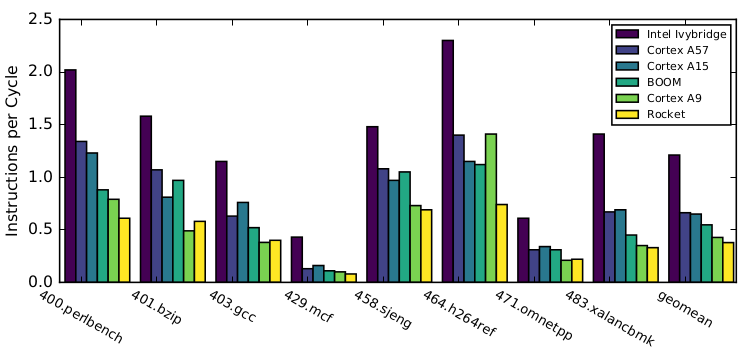
\includegraphics[width=\textwidth]{IPC_spec2006}
			\caption{}
			\label{fig:ipc_cmp_fig}
		\end{subfigure}
		\begin{subfigure}[b]{0.8\textwidth}
			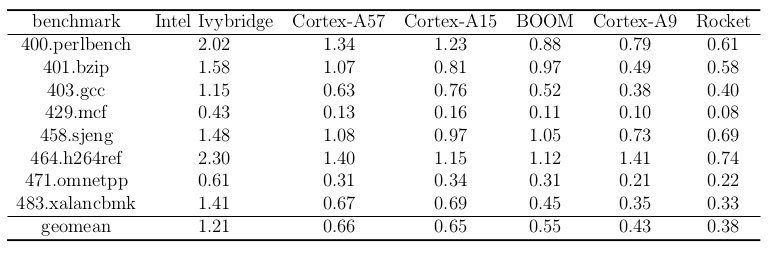
\includegraphics[width=\textwidth]{IPC_num}
			\caption{}
			\label{fig:ipc_cmp_tbl}
		\end{subfigure}
		\bicaption{SPECint2006 IPC不同IPC比较。(a) 图。\citep{Celio:EECS-2018-151}图3.7. (b) 表。\citep{Celio:EECS-2018-151}表3.6.}{Instruction-per-cycle comparison running SPECint2006. (a) The figure of instruction-per-cycle comparison running SPECint2006, Figure 3.7 of \citep{Celio:EECS-2018-151} (b) The table of instruction-per-cycle comparison running SPECint2006. Table 3.6 of \citep{Celio:EECS-2018-151}}
		\label{fig:ipc_cmp}
	\end{figure}

	虽然1.35已经是个不错的成绩,但是,是基于icache全部命中,没有访存延迟,而且转移预测器命中率达到97\%以上的前提下。在一般的情况下,可想而知连1都很难达到。对比图\ref{fig:ipc_cmp}中当前成熟处理器的性能,还有很大的性能提高空间。既然指令宽度为2的超标量顺序执行已经达到瓶颈,很自然地脑海中会浮现出三种方案:
	\begin{enumerate}[label=(\alph*)]
		\item 继续提高取指宽度,比如四条指令的超标量,后端继续做顺序。
		\item 不提高取指宽度, 因为对于指令宽度为2,前端供应指令的最大IPC可以达到1.8。计算方法为:每周期指令最多是2条,假设跳转指令占总指令的20\%,跳转指令在第一条位置的概率是50\%,跳转目标在第一条指令的概率是50\%,预测单元全部猜对,最后计算得到每周期正确的指令为1.8条。从1.33到1.8还是有较大的提升空间,所以后端可以采用乱序微结构来做指令的动态调度。
		\item 即增加取指宽度,又把后端做成乱序。
	\end{enumerate}

	权衡三个方案: 第一个反而是最不切合实际的,换言之与高性能的目标背道而驰。宽度为4的取指器要在已有的取指器的基础上改成4条指令宽度,由前面的分析,电路逻辑复杂,时序不好,对转移猜测极不友好。其次,从FUXI的IPC瓶颈的分析中,可以看出,真正的瓶颈不在于前端而在于顺序执行的后端。那么第三个方案呢,也不切合实际,主要是因为目前,是从来没有设计过乱序处理器的新人,水平有限。比较之下,第二个方案是最合适的。

综上分析,最后毕业设计的处理器核心具体的结构就是取指宽度为2的前端匹配上乱序执行结构的后端。

\section{中间层的引入}\label{subsec:middle_end}
事实上,前后端的设计思想最初应该是借鉴于编译原理的。编译原理作为计算机领域一门成熟学科,就是通过前后端的设计方法学来降低编译器设计的复杂度。类比于只采用前后端模型的简单编译器,对于简单的顺序执行的五级流水,前后端的划分也是足够的。但是为了做代码优化,编译原理专门提出了中间表示层的概念,依托清晰的结构化设计,再一次的有效地控制了问题的复杂度。而这一思路同样可以借鉴在结构上比顺序更复杂的乱序处理器的设计上。事实上,在乱序的处理器中,要从顺序的前端变化到乱序后端,最后再从乱序的执行变回顺序的提交,恰好需要有这么一个像中间桥梁一样的中间层的存在。

\section{处理器的状态}\label{subsec:cpu_state}
章节\ref{subsec:middle_end}中提到了引入中间层的必要性。而如果用一句话来概括中间层的作用,那就是管理处理器状态的变化。那么什么是处理器的状态。指令和访存的数据是外部来的激励,算不上是处理器的内部状态。所以只有PC值,32项数据寄存器值能算是处理器状态。站在更高的视角来看,所有处理器的物理数据结构,外来的指令数据最后修改的都只有这两类寄存器。而套用前后端的模型,前端管理PC,后端管理32项数据寄存器,中间层则是管理这些状态的变化。

\section{指令乱序调度和执行级别}\label{subsec:exe_hierarchy}
论及乱序指令调度,这样的机制虽然做到后面准备好的指令可以先于前面没有准备好的指令执行,但也不意味着要做到真正意义上的毫无差别调度最先准备好操作数的指令,哪怕这条指令距离最早未提交指令的64条开外。为了支持在这个例子里所说的远在64条开外的指令的乱序调度,所付出的硬件的代价对于效率的收益值不值得,是值得商榷的。但它一定不是一个好的设计思路,因为它没有体现出一种被体系结构所强调的思想 --- 层次化。就拿最为经典的存储结构来说,从处理器内部的寄存器堆,到一级高速缓存,二级高速缓存,共享缓存再到内存,硬盘,磁盘,好的设计是把越重要越常用的数据放在越快速的存储设备中的,而不会是因为寄存器堆很快速就去把寄存器堆做达到百兆的容量。换言之分清主次的层次化才是真正好的设计,处理器的设计亦是如此。所以,在毕业设计中特别强调,对指令调度乱序执行要有等级化、层次化的划分。

回想在顺序流水的设计中,其实同样有指令的执行等级划分,只不过做的很极端而同样不合理 --- 处在流水线越下游的指令执行级别越高,而且这种级别精确到每一条指令,只要下游早的指令没有执行完或者没有准备好操作数,上游的所有指令都不能执行。这就是顺序执行自带的而且无法改变的执行等级划分的通病。如果以这种角度来思考,乱序能带来了什么?带来的是可以打破这种僵硬的等级划分通病,带来的是可以自行定义执行等级的自由。当然这种自由是靠更多的硬件资源交换得来的,来之不易就不能随意挥霍。需要对执行等级的自定义深思熟虑,做到符合指令执行的规律,这样才会高效。

大方向的规律非常清晰,就是越早被取回的指令,执行等级越高,被优先执行的倾向越大,反之执行的等级越低。但是又不能像顺序一样走向极端。所以等级一定是按照指令新旧的梯队来划分的,如第一梯队,第二梯队等等,然后每一梯队里面包括了不止一条的若干条指令集合。就以BIAN处理器中具体体现出层级化的设计点举例来说,BIAN微结构上将指令的执行等级分为3级:
\begin{enumerate}[label=(\alph*)]
	\item \textbf{第一梯队的指令集合}:容量$2 + 2 + 2 + 4 = 10$条,参见图\ref{fig:bian_over1}。其中两条位于从重命名阶段到执行阶段的锁存器中,其他8条分别位于3个执行队列中。每条指令都存储住两个操作数,不需要再次读寄存器堆,侦听到写回总写结果立马可以在每个队列中选出最早的一条指令执行,分配有一个通用的ALU,和一个写回端口。相当于是两个输入三个输出的执行调度站,详细的调度策略参见章节\ref{subsec:execute_q}。
	\item \textbf{第二梯队的指令集合}:容量$ 9\times 2 = 18$条,是两个容量都为$ 8 + 1 $条指令的并行的发射队列,其中8条位于8项移位队列中,1条头部寄存器中,这样的设计时序会比直接9项的移位队列更好。队列中的每一项通过侦听前递信息判断操作数准备与否。位于队列中的指令会先移到头部;位于头部指令会和旁路过来的流水线二三级之间锁存器中的指令做二选一的逻辑,读寄存器堆获得源操作数,进入执行阶段。
	\item \textbf{第三梯队的指令集合}:容量$ 16\times 2 = 32$条,存储结构为循环队列,每一项可容纳两条指令。指令顺序出队列进入重命名阶段。容量最大,执行级别最低。
	\item 还有另外一类指令不好纳入这三个梯队中,由于功能特殊,而且是对外的操作,需要单独占有一个写回端口,这就是访存指令。这类指令对于处理器性能的影响很大,所以需要着重优化,我的设计中采用的是非常经典的LDQ和STQ分别存放load和store类指令的信号,参见图\ref{fig:ls_unit},目前的参数分别都是6项。同时为了提高访存密集型程序的性能,另外专门设计了一个可以同时存放load,store指令的load/store队列,里面只存放了很少量的关于访存指令的信息。作为比LDQ和STQ执行等级更低的存储单元以避免因为LDQ和STQ容量太小而导致频繁阻塞前端指令供应的情况。具体的设计考虑参见章节\ref{subsec:ls_queue};具体的运作机制参见章节\ref{subsec:ls_unit}。
\end{enumerate}
\subsection{总结}

如果保守估计在LDQ和STQ中共分担4条访存指令,那么乱序执行的指令总数可达$ 10+18+4 = 32 $条,在乱序执行的上游还可以有32条的顺序的指令缓存(第三梯队)。所以处理器中可以最多容纳64条指令,两条并行的发射队列(第二梯队),加上3条并行的执行队列(第一梯队)。另外,一共有3个ALU运算部件;寄存器堆有4个读端口,4个写端口,读写端口较少,特别是读端口数量是双发射架构中最少的。整个处理器架构如图\ref{fig:ls_unit},设计合理。
\begin{figure}[!htbp]
	\centering
	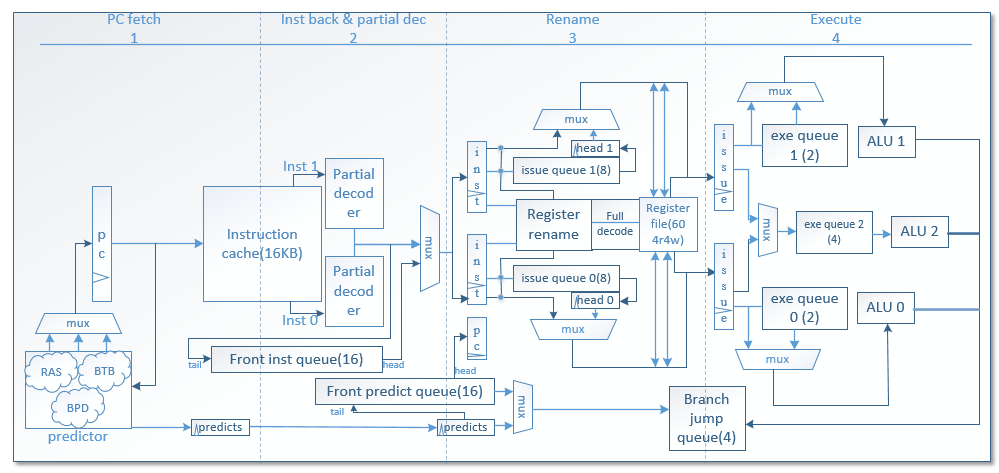
\includegraphics[width=\linewidth]{bian_overview}
	\bicaption{BIAN处理器整体框图,不包括访存单元}{Block diagram of BIAN processor (not include load-store unit.)}
	\label{fig:bian_over1}
\end{figure}

\begin{figure}[!htbp]
	\centering
	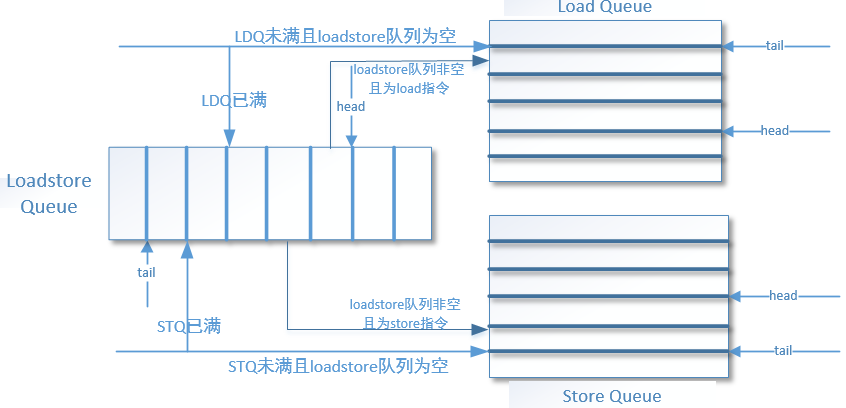
\includegraphics[width=\linewidth]{load_store_unit}
	\bicaption{BIAN处理器访存单元}{Block diagram of load-store unit in BIAN processor.}
	\label{fig:ls_unit}
\end{figure}

\section{流水线阶段划分}
%TODO 用了很多bypass的技巧
处理器流水级的划分如图\ref{fig:my_pipeline}:
\begin{figure}[!htbp]
	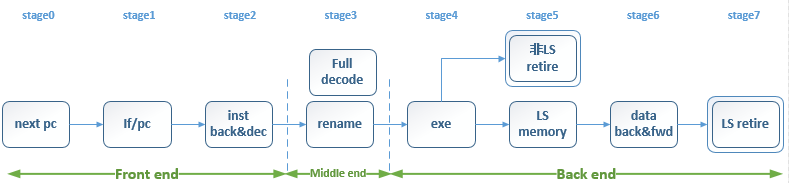
\includegraphics[width=\linewidth]{pipeline_stage}
	\bicaption{BIAN处理器的流水线示意图。}{the pipeline of BIAN processor.}
	\label{fig:my_pipeline}
\end{figure}
\begin{enumerate}[label=(\alph*)]
	\item 第0级 --- \textbf{next\_pc级}
	
	界定有没有这一级的标准是对于后端得到的跳转地址以及跳转使能信号,是直接送到pc级(稍后要介绍的第1级)向内存或icache发出PC,还是先送到锁存器锁存一个周期,再送到pc级。概括起来前一种做法是组合逻辑,后一种做法是时序逻辑。组合逻辑没有第0级,优势在于如果转移猜测错误,浪费的周期数会比时序逻辑要少一拍,最为极端的例子是在带有延迟槽的ISA如MIPS,最简单的单发射五级静态流水采用组合逻辑的方案从而不需要转移猜测。但是组合逻辑的劣势也是很明显的,就是时序不好,从后端计算出来直接跳转目标和有PC以及各级转移猜测的目标地址做多选,最后得到发出的PC值。pc级电路延迟很大,导致一方面访问icache的时序紧张,另外一方面如果要做转移猜测,那么PC值还要连到转移预测单元中得到下一周期PC值。这样就会把整个pc级撑得很大,对整个CPU的频率做高不利。所以本质上来讲,next\_pc级是为了缓解pc级的压力而增加的一级。
	\item 第1级 --- \textbf{if/pc级、取指级}
	
	发出PC从内存或者icache中取指,和经典的五级流水线保持一致。
	\item 第2级 --- \textbf{inst back \& dec级,译码级}
	
	这一级的名称兼容于经典的五级流水,原来的含义是指令在这一级被取回然后译码得到处理器内部操作微码。但是在BIAN处理器中,这一级只需做部分译码,得到一些简单的如是否是跳转指令的信息,从而减小这一级的电路延迟。再者,BIAN不会在接下来的第3级立刻执行指令,全译码放到第二级的需求不大。
	\item 第3级 --- \textbf{rename级、重命名级}
	
	这一级是BIAN处理器中至关重要的一级,承接着前端与后端,管理着后端的各种资源。从前端的角度来看,这一级还可以进行更加复杂策略的转移猜测;从后端的角度来看,这一级完成从逻辑寄存器到物理寄存器的转换和指令所需物理资源的分配。这里的物理资源有物理寄存器、内部指令标识符id号、也即reorder buffer的id号、访存队列、分支跳转队列、发射队列。读同步寄存器也在重命名级进行。
	\item 第4级 --- \textbf{execute级、执行级}
	
	在执行队列或者旁路过来的发射指令,选出3条准备就绪的指令在3个ALU中运算执行,如果是单周期ALU指令,写回寄存器堆;若是分支跳转指令发送到分支跳转单元;若是访存指令送到访存单元中。
	\item 第5级 --- \textbf{非LS retire级/LS memory级}

	乱序处理器流水级的划分从这级开始分化。单周期的ALU指令已经是retire级了,因为所需操作已经做完,在ROB中进行相应的提交操作就可以退出。但是对于访存类的指令,这一级是memory级,进行的操作是向内存发出访存地址和load请求。
	\item 第6级 --- \textbf{data back \& forward级}
	
	load所需的数据将在这一级被取回,同时做forward操作,将位于该load指令之前所有未写回内存,且与该load指令地址冲突的store指令的数据前递到load的数据中。成功加载到内存数据便可写回寄存器堆。
	\item 第7级 --- \textbf{LS retire级}
	
	对于load指令,在ROB中提交就可退出;对于store指令,当ROB队列的头部id号等于STQ的头部store指令id号时,将数据写回内存,并且移动ROB队列的头指针。退出处理器。这一过程中还会做backward操作 --- 检测位于该store指令之后是否有地址有冲突同时尚未做前递便已经将数据加载写回的load指令,若有,前端会以这条load指令的PC值为起点重新开始取指,做回滚操作。
\end{enumerate}
	\subsection{总结}
	访存指令从第0级到第7级完成提交退出,一共要经历8个周期,这是BIAN处理器指令流的最长路径。从前后端的模型来看,第0级到第2级的前3级流水属于前端(front end),第4级到第7级的后四级流水属于后端(back end),第3级单独成为一层 --- \textbf{中间层}(见章节\ref{subsec:middle_end})。
	
\section{前端的设计}
前端包括取指单元,转移预测单元和一级高速缓存。下面从这三个单元来剖析:
\subsection{取指单元}
从最简单的宽度为1的取指单元开始设计,代码如下:
\begin{scala} 
	/*一共有3个状态:
	* sWtAddrOK状态下等待地址握手成功
	* sWtInstOK状态下等待指令取回
	* sWtForward状态下等待后端接收取回的指令
	*/
	val sWtAddrOK :: sWtInstOK :: sWtForward :: Nil = Enum(3)
	val state = RegInit(sWtAddrOK) //取指单元的初始状态
	switch (state) {
		is (sWtAddrOK) { //在sWtAddrOK状态下
			//如果地址握手成功,切换到sWtInstOK状态
			when(addr_ready) { state := sWtInstOK }
		}
		is (sWtInstOK) { //在sWtInstOK状态下
			//若外界发送的指令有效,意味着指令被顺利取回
			when(inst.valid) {
				when(io.forward || inst_kill) { //被接收或者被取消,判断地址是否握手成功进入相应的状态
					state := Mux(addr_ready, sWtInstOK, sWtAddrOK)
				}.elsewhen(io.dec_kill) { //如果被流水线下游取消掉取回来的指令,切换到sWtAddrOK重新开始地址握手 
					state := sWtAddrOK 
				}.otherwise { //如果后端暂时无法接收,切换到sWtForward状态
					state := sWtForward 
				}
			}
		}
		is (sWtForward) { //在sWtForward状态下
			when(io.forward) { //被接收,判断地址是否握手成功进入相应的状态
				state := Mux(addr_ready, sWtInstOK, sWtAddrOK)
			}.elsewhen(io.dec_kill) { //如果被流水线下游取消掉取回来的指令,切换到sWtAddrOK重新开始地址握手
				state := sWtAddrOK 
			}
	}	}
\end{scala}
上面的代码就是描述整个取指器行为的状态机,一共只有3个状态,非常的简洁清晰,可以用图\ref{fig:fsm_fetchi}来描述:
\begin{figure}[!htbp]
	\centering
	\begin{tikzpicture} [->,>=stealth',shorten >=1pt,auto,node distance=3.5cm,
	semithick]
	\node[state, accepting, fill=green](q0) {\tiny{sWtInstOK}};
	\node[state, below left of=q0, initial,fill=green] (q1) {\tiny{sWtAddrOK}};
	\node[state, accepting, below right of=q0,fill=red](q2) {\tiny{sWtForward}};
	
	\path
	(q1) edge[bend right] node{\scriptsize{addr\_ready}} (q0) 
	edge[loop below] node{\scriptsize{!addr\_ready}} ()
	
	(q0) edge[bend right] node[swap]{\scriptsize{!addr\_ready \&\& \dots}} (q1) edge[bend right] node{\scriptsize{!io.forward \&\& \dots}} (q2) edge[loop above] node{\scriptsize{!inst.valid || addr\_ready \&\& (io.forward || inst\_kill) }} ()
	
	(q2) edge[bend right] node[swap]{\scriptsize{io.forward \&\& addr\_ready}} (q0) edge node{\Longstack[l]{\scriptsize{io.forward \& !addr\_ready} \\ \scriptsize{|| io.dec\_kill}}} (q1)
	edge[loop below] node{\scriptsize{!io.forward || !io.dec\_kill}} ();
	\end{tikzpicture}
	\bicaption{取指单元的有限状态机。}{the FSM of FetchInst Unit.}
	\label{fig:fsm_fetchi}
\end{figure}

除了简洁的状态机模型,取指单元还做了两点设计:
\begin{enumerate}[label=(\alph*)]
	\item 在电路频率的考虑上,将所有从后端和内存传来的信号,都用锁存器锁存一个周期再去改变取指单元的状态,从而保证了取指单元的时序和外界独立。
	\item 为了配合图\ref{fig:fsm_fetchi}中的三个状态的状态机,取指的逻辑上有一个最为基本的限定 --- 取指的in-flight指令数最多为1。取指单元和icache都要相应地做成阻塞式,也即要等到正在访问内存或者icache的PC对应的指令被取回并被后端接收,才能够发出下一个PC取指请求。这种只能跟踪一条PC取指的方式,严格保证了取指的顺序性,同时取指单元的效率又不会有明显的损失。
\end{enumerate}

接下来是将取指单元的宽度从1提高为2,实现超标量。可是这个跨越并不简单。首先必须摆脱的误区是,由于内存的端口宽度是限定为1条指令32位的,所以如果直接访问内存,那么一个周期内取回的指令宽度仍然是1而不是2。故icache miss后burst传输是逐条指令传输回来的。宽度为2的情况只会出现在icache命中的情况下。这样,超标量的取指单元为了保证效率,显然不能等到可以两条指令同时从cache取回来的时机。Burst传输和uncacheable下直接访问内存的情况都要做到取回一条指令就立即发出一条指令。这样也可以理解为能够支持单宽度和双宽度之间的来回切换。得益于上述in-flight指令数最多为1的基本限定,双宽度的取指单元仅仅需要在原有的单宽带的基础上稍加修改。相比单宽度,双宽度有以下几个需要多考虑的逻辑:
\begin{enumerate}[label=(\alph*)]
	\item 超标量的两条指令是2对齐的,第一条指令一定是偶数PC,第二条一定是奇数PC。如果if/pc级发出偶数的pc,然而dec级由于cache miss再通过burst传输先传回了第一条偶数的指令,这时候可以不用顾及后端给出的forward接收信号,立马发出后一条的奇数PC取指。这个考虑使得无论再什么样的情况下,双宽度的取指效率都不会低于单宽度的取指效率。
	\item 指令流会有跳转,而且有一半的概率是在第一条指令的后面需要跳转(有预测单元给出),这种情况在BIAN的设计中被称为inst split,上述代码中用inst\_split变量来表示,如果第二条指令也取回来了,要取消掉。
	\item 当出现inst split的情况,而且预测单元给出的目标地址是奇数PC时,取指单元可以同样不用顾及后端的forward接收信号,直接发出跳转目标地址去取指。这样能进一步地继续提高取指效率。但是会存在子啊一个周期里被后端接收的指令不是地址连续的情况,这一点需要注意。
	\item 后端的forward接收信号变成了两位向量,使得并行的两条指令被后端接收变得独立。
\end{enumerate}

呈现的状态机代码如下:
\begin{scala}
	val sWtAddrOK :: sWtInstOK :: sWtForward :: Nil = Enum(3)
	val state = RegInit(sWtAddrOK)
	val inst_valid_orR: Bool = inst_valid.reduce(_||_)
	/*if_forward变量添加,是双宽度和单宽度之间最主要的不同
	* 表示的意义是当状态在sWtInstOK而且指令取回时,
	* 能够继续发送PC取指请求的集中不同的条件
	* 或表达式的最后一项的Mux多选逻辑参考
	* 前面双宽度需要多考虑逻辑的(a)(b)(c)部分
	*/
	val if_forward: Bool = io.forward(1) || inst_kill || Mux(inst_split, io.pc(conf.pcLSB).toBool, !inst_valid(1))

	switch (state) {
		is (sWtAddrOK) {
			when (addr_ready) { state := sWtInstOK }
		}
		is (sWtInstOK) {
			when(inst_valid_orR) {
				when(if_forward) { // almost the only difference
					state := Mux(addr_ready, sWtInstOK, sWtAddrOK)
				}.elsewhen (io.dec_kill) { state := sWtAddrOK
				}.otherwise { state := sWtForward }
			}
		}
		is (sWtForward) {
			when(io.forward(1)) {
				state := Mux(addr_ready, sWtInstOK, sWtAddrOK)
			}.elsewhen (io.dec_kill) { state := sWtAddrOK }
		}
	}
\end{scala}

\subsection{cache core设计}\label{subsec:cache_core}
数据和控制应该相互独立。这是为什么cache core和icache分开论述的原因。Core可以有不同的数据组织形式 --- 直接映射、全相连、多路组相连。同样,多路的时候可以有不同的替换算法。但这一切都与读写的逻辑无关,对外呈现的读写端口不变。只要求cache行的长度对外保持一致即可。将数据和控制逻辑解耦和,可以做到最大程度控制复杂度。另外一方面也可以做到逻辑的复用。比如icache和dcache对于读写的控制逻辑不一样,但是cache core的存储结构可以做到一致。虽然目前BIAN处理器仅是用一个16KB的直接映射组织结构来代替四路组向量每一路4KB的组织结构,但是由于数据和控制的分离,控制的逻辑无变动,对数据结构的修改其实并不困难。

\subsection{指令高速缓存}
Icache状态机的代码如下:
\begin{scala}
	val sLookUp :: sBurst :: sWriteBack :: Nil = Enum(3)
	val state = RegInit(sLookUp)
	switch (state) {
		is (sLookUp) {
			when (pc_miss) { state := sBurst
			}.otherwise { state := sLookUp
		}
		is (sBurst) {
			when (rlast && rvalid) { state := sWriteBack
			}.otherwise { state := sBurst }
		}
		is (sWriteBack) {
			when (pc_double_miss) { state := sBurst
			}.otherwise { state := sLookUp}
		}
	}
\end{scala}
\begin{figure}[!htbp]
	\centering
	\begin{tikzpicture} [->,>=stealth',shorten >=1pt,auto,node distance=3.5cm,
	semithick]
	\node[state, accepting](q0) {\tiny{sBurst}};
	\node[state, below left of=q0, initial, accepting] (q1) {\tiny{sLookUp}};
	\node[state, below right of=q0, accepting](q2) {\tiny{sWriteBack}};
	
	\path
	(q1) edge[bend left] node{\scriptsize{pc\_miss}} (q0) 
	edge[loop below] node{\scriptsize{otherwise}} ()
	(q0) edge[bend right] node[swap]{\scriptsize{rlast \&\& rvalid}} (q2) 
	edge[loop above] node{\scriptsize{otherwise}} ()
	(q2) edge[bend right] node[swap]{\scriptsize{pc\_double\_miss}} (q0) 
	edge node{\scriptsize{otherwise}} (q1);
	\end{tikzpicture}
	\bicaption{Icache的有限状态机。}{the FSM of Icache.}
	\label{fig:fsm_icache}
\end{figure}

如图\ref{fig:fsm_icache},状态机一共有3个状态。sLookup阶段,在icache中以PC的低位为索引查PC对应的指令是否命中,如果出现miss了就进入sBurst状态进行burst传输。burst传输是AXI协议中的一种传输模式(但也不局限于AXI协议,很多高新能的总线协议中都有类似的模式),发出一个PC,能够取回这个PC所在的一段连续指令。比方说burst的长度设置为16,即使cache miss,在一段访问内存的延迟后,也有16个周期是有指令可以提供的,这样就能够大大降低访存延迟的代价。

BIAN的icache把burst传输长度设置为16,与cache行长度吻合。在AXI协议中burst有着两种基本的模式,一种是INCR,一种是SWAP。通俗来说INCR就是在以PC为起点,往后取一段指令,所以INCR发出的PC一般要指令长度对其。SWAP同样是以PC为起点,但是PC不要求是指令宽度中最前段的指令,可以是中间的某条指令,向后取指到达右边界后再循环到左边界直到取回来PC的前一条指令。icache采用的是INCR模式,因为其一取指有连续的倾向,而且在很大的情况下导致burst传输的pc都是cache行的第一条,虽然SWAP模式一定不会比INCR差,但是SWAP模式其实和INCR效率相差不大;另外,考虑到取值时序紧张,INCR模式对内对外都比SWAP模式友好。故最后采用的INCR模式。

回到状态机上,当状态是sBurst时,如果rlast和rvalid信号同时置上了,说明最后一条指令也被取回来了,状态就会跳到sWriteback状态。sWriteback状态下就是把取回来暂时用锁存器缓存的整个cache行写回章节\ref{subsec:cache_core}的存储结构中。为了提高效率,在burst传输阶段也是同步可以接收取回来的指令的,这样就会出现可能一个跳转出现第二次的PC在cache中的miss,这个时候整个取指单元就会因为in-flight取指数至多为1的基本限定而卡住动不了了。故在sWriteback状态下,如果检查到PC的二次miss就会直接进入sBurst传输阶段,从而提高效率。如果没有出现二次miss,那么就会又跳回sLookup状态。整个icache的行为简洁而高效。

\subsection{转移预测单元}
除了高速缓存技术,转移猜测也是高性能处理器的关键。与简单的流水线后端一遇到阻塞就要暂停前端取指不同,高性能的处理器一定是要做到后端遇到阻塞如访存数十拍的延迟时,还能允许前端继续投机地取指。来不及处理的指令将会被缓存在后端。按照转移指令在程序中15\%左右的占比,意味着指令流会在平均6$ \sim $8条之后可能重定向一次,如果没有转移猜测,一味的增加PC,等到前面的跳转指令被执行确认指令流需要重定向,那么后面的指令会被取消掉,体现不出指令缓存的作用,浪费存储面积。要真正发挥缓存指令的优势,就必须依赖转移猜测来提高缓存指令的正确性。转移预测可以分布在流水线的如下阶段:
\begin{enumerate}[label=(\alph*)]
	\item if/pc级要得到下一周期取指PC,此时还不知道PC对应的指令是不是跳转指令,唯一有用的信息是根据历史存储的从PC到目的地址的映射。但是PC有32位,靠RAM来索引不符合实际,剩下的方案只剩CAM表。代表性的数据结构是BTB,参见章节\ref{subsec:BOOM}。CAM表只能存少数的映射关系,比较理想的是32$ \sim $64个。在BIAN处理器中实现了用BHT和gshare算法辅助预测分支跳转方向,64项BTB映射表,能够存储64条分支跳转的目标地址。
	\item inst back级指令已经取回,但是整个周期剩余不了多少时间,最多只能根据局部译码检测到是函数返回指令选择RAS(参见\ref{subsec:BOOM})的栈顶地址重定向指令流。而在目前的BIAN处理器中,并没有实现在这一级基于RAS的转移预测,而是先锁存了一个周期,在rename级做。
	\item rename级中,对于简单的jal/j指令,可以直接由对应的PC和指令中的立即数域得到跳转地址并进行指令流重定向;对于branch类指令,虽然能够算出跳转地址,但尚不知道跳转方向。可以使用BHT和章节\ref{subsec:alpha}中提到的基于local历史和global历史的锦标赛预测机制来预测方向。目前,在BIAN的实现中,这一级仅仅做了jal/j指令以及对未在if/pc级未做预测的branch类指令的跳转。正在准备添加这段逻辑来提高预测率和处理器整体的性能。
\end{enumerate}

\subsection{预测单元优化}
在处理器的设计当中,有很多关于效率,时序,面积的权衡,这在预测单元的设计中得到了充分地体现。预测单元采用更加复杂的预测技术把预测正确率做到更高的同时,要付出更多的面积,更长的电路延迟和更大的功耗。在保证预测正确率的基础上,对于面积时序的优化也显得重要。下面突出在BTB结构中BIAN处理器所做的优化:

BTB原理简单,但是却是转移猜测中最为重要的一个部件,直接分担了程序跳转80\%左右的预测正确率。这个逻辑上简单的从pc到target的映射关系,值得好好的分析得到更好的物理实现,保证容量和正确率的同时降低面积和延迟的开销。
\begin{enumerate}
	\item 观察一:在映射关系中,无论是PC还是target的高位很少有变化,所以一个想法就是能不能把高位比如说高16位和低位比如低16位分开,做成两个表的映射。这样考虑到高位很少变动,高位的映射表项数就可以做的很小,比如4项(低位还是64项),如图\ref{fig:btb_opt1}。计算一下,采用这种的设计方案,总共占用的面积是$ 4\times16\times2 + 64\times16\times2 + 64\times2 = 2304 = 36\times 32\times 2 $ bits。最后加的$ 64\times2 $是在低位映射表中存储高位映射表的索引号所需要的面积,这个相当于36项32位PC映射到32位target的直接映射表。当然,如果是64位的ISA下,这种优势会更加明显。那么电路延迟如何呢?面积一样的情况下,两张CAM表的延迟不会比一张CAM表差,反而会因为面积减小,电路的布局布线上有优势。
	\begin{figure}[!htbp]
		\centering
		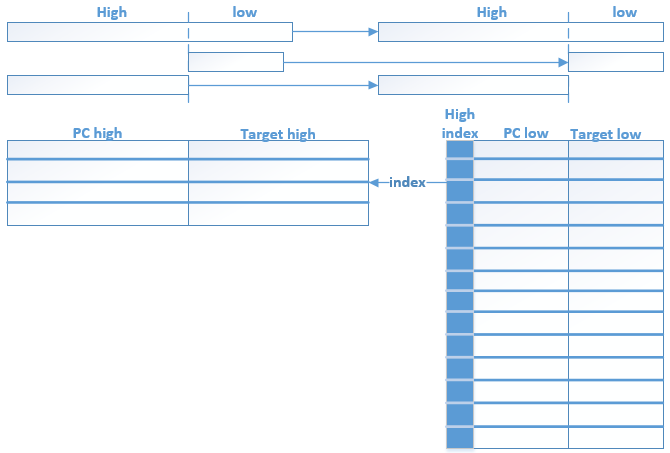
\includegraphics[width=0.6\linewidth]{btb1}
		\bicaption{观察一引出的物理数据结构的优化。左侧为高位映射表,右侧为低位映射表}{the physic data structure optimization by observation one. The left is the high bits map table, the right is the low bits map table.}
		\label{fig:btb_opt1}
	\end{figure}	
	\item 观察二:PC到target的映射中高位基本上都是一致的,也就是说程序的行为大多数都是在小范围内相对跳转。针对这一特点,在低位的映射表中再加1-bit的标志位,标记映射的高位是不是相等,如果高位相等就不需要占用高位映射表项,大大降低了高位映射表的替换率,从而提高了优化一数据结构的预测稳定性,如图\ref{fig:btb_opt2}。
	\begin{figure}[!htbp]
		\centering
		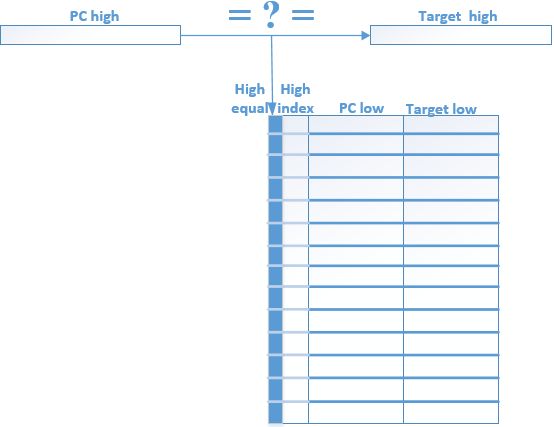
\includegraphics[width=0.6\linewidth]{btb2}
		\bicaption{观察二引出的物理数据结构的优化。只包含了低位映射表。}{the physic data structure optimization by observation two. Only include the low bits map table.}
		\label{fig:btb_opt2}
	\end{figure}
\end{enumerate}

\subsection{前端部件的整合}
上面讲述了前端的各个组件,这些组件整合起来构成了整个处理器BIAN的前端,如图\ref{fig:frontend}。
\begin{figure}[!htbp]
	\centering
	\begin{tikzpicture}[
	node distance = 12mm and 30mm,
	->,>=stealth',shorten >=1pt,semithick,
	box/.style = {rectangle, draw, fill=#1, 
		minimum width=12mm, minimum height=7mm}
	]
	
	\node (n1) [box=green] { next\_pc };
	\node (n2) [box=green,right=of n1] {if/pc};
	\node (n6) [box=white,below=of n2] {RAS};
	\node (n7) [box=white,above=of n2] {BTB};
	\node (n3) [box=green,right=of n2] {instback};
	\node (n4) [box=green,right=of n3] {rename};
	\node (n5) [box=white,below=of n4] {decoder};
	%
	\draw[->] (n1) to ["io.pc\_forward"] (n2);
	\draw[->] (n2) to ["pc\_valid"] (n3);
	\draw[->, swap] (n3) to ["io.inst.valid"] (n4);
	\draw[->, bend left] (n4) to ["io.forward"] (n3);
	\draw[->, bend right,swap] (n4) to ["io.if\_kill"](n2);
	\draw[->, bend right] (n4) to ["io.dec\_kill"] (n3);
	\draw[->] (n4) to ["inst"] (n5);
	\draw[->] (n5) to ["stack push and pop "] (n6);
	\draw[->] (n6) to ["peek"] (n2);
	\draw[->] (n7) to ["predict", swap] (n2);
	\end{tikzpicture} 
	\bicaption{处理器BIAN的前端流水线。}{the pipeline of frontend.}
	\label{fig:frontend}
\end{figure}

整个前端是一个三级流水,因为指令in-flight的请求至多为1的基本限定,十分简洁。主要体现在流水线的3大控制信号上:\texttt{io.pc\_forward}是控制取指PC从next\_pc级流向if/pc级的使能信号;\texttt{pc\_valid}是控制取指PC和BTB预测信息从if/pc级流向dec级的使能信号;\texttt{io.inst.valid}是控制取回指令和地址预测信息从dec级最后流向后端rename级的使能信号。这3级流水的阻塞与流通可以简单的解释为:首先最靠近后端的dec级如果在\texttt{io.inst.valid}和\texttt{io.forward}同时置上的时候,才能被后端接收,下一周期空出这一级,而if/pc级的信号要流向dec级须等dec级在下一周期能够被空出来,同理next\_pc级的信号要流向if/pc级须等if/pc级在下一周期能够被空出来。

相比于单宽度的前端,双宽度的前端还需要额外考虑两条并行的指令之间的干扰现象,具体来说是第一条指令对第二条指令的影响。在前端流水线的3级中:
\begin{enumerate}
	\item \textbf{if/pc级},虽然对外的取指端口是一个PC,但是这个时候对内的PC已经分化成奇偶两个。在BTB的结构中,如果第一条PC命中,并且方向为跳转,那么第二条的PC就会被无效掉。这一级的干扰现象被支取单元所解决。
	\item \textbf{inst back级},为了使得后端的逻辑简单化,通过局部译码,得到如果两条并行指令都是特权指令或者都是分支跳转指令时,就会阻塞该级流水,使两条指令串行发送给后端。
	\item \textbf{rename级},转移预测单元若在该级的第一条指令上纠正了流水线上游传输过来的预测信息,同样要将与之并行的第二条指令无效掉。
\end{enumerate}

\section{中间层的设计}

中间层承接着处理器的前端和后端。前端的前端指令队列、分支跳转预测队列的出口;后端的指令发射队列、分支跳转单元队列和访存队列的入口均位于中间层。中间层还专门负责管理处理器的状态变化与恢复,并能够按照每条指令的不同需求,精确地分配各个物理资源。是乱序处理器中最为重要的结构之一。

中间层涉及了很多部件单元。不过在论述每个具体部件之前,不妨先分析清楚承载这些功能单元的基本数据结构 --- 队列。

队列在电路中如图\ref{fig:queue}有两种实现形式:
\begin{enumerate}[label=(\alph*)]
	\item \textbf{循环队列},依靠着头尾两组指针来控制逻辑。称之为``组'',是由于考虑到同时入队列和同时出队列可能不止一项。入队列移动尾指针,出队列移动头指针。
	\item \textbf{移位队列},只需要依靠一个计数器来记录当前队列中有多少项即可。入队列从队列的尾部依靠计数器的指示进入;出队列项的后面诸项需要向前移位来填补出队列的空白。
\end{enumerate}
\begin{figure}[!htbp]
	\centering
	\begin{subfigure}[b]{0.45\textwidth}
		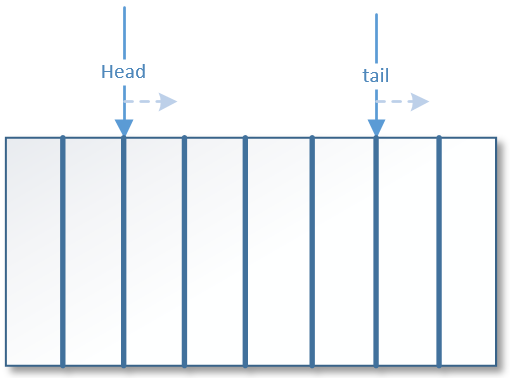
\includegraphics[width=\textwidth]{ring_queue}
		\caption{}
		\label{fig:ring_queue}
	\end{subfigure}
	~
	\begin{subfigure}[b]{0.45\textwidth}
		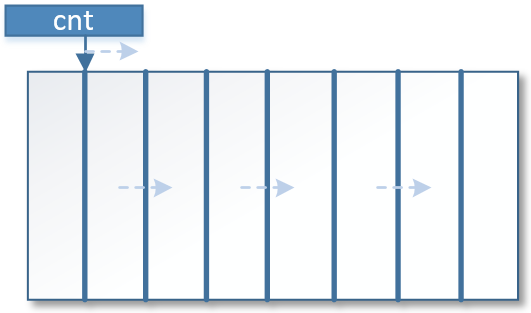
\includegraphics[width=\textwidth]{shift_queue}
		\caption{}
		\label{fig:shift_queue}
	\end{subfigure}
	\bicaption{两种类型的队列。(a) 循环队列,(b) 移位队列。}{Two types of queue. (a) Ring queue, (b) Shift queue.}
	\label{fig:queue}
\end{figure}

这两种不同的形式各有优势。循环队列对于出入队列的项数约束较松;移位队列入队列的项数约束较松,但是对于出队列的项数约束较严,一项是最为简洁的。项数一旦大于1,复杂度就会明显地提高,物理实现变得复杂,同时移位队列的功耗比循环队列大很多,因为移位队列平均1/2项数都会变移动,而循环队列只需要移动头尾指针。

但是循环队列并不适合承载乱序的逻辑,这是由其逻辑特性决定的,出队列项一定是头指针所指向的;与循环队列相反,移位队列非常适合承载乱序的逻辑,队列中的任何一项都可以出队列,留下的空位由后面项移位来补。同时,乱序中的多项同时可以出队,只选最早一项的逻辑,用移位队列来实现显得非常简单,只需要调用优先编码器,传入可以被发射的队列向量,最后按照优先级得到的独热码对应的就是应该出队列的最早一项。

但是移位队列的功耗毕竟太大,特别是每一项位数很大的时候。出于降功耗的考虑,对移位队列的结构做了优化如图\ref{fig:opt_shift_q}所示,只将能够决定出队列条件的最关键控制信号填入移位队列中,其他的数据信号则填入到数据表中,然后把该表项的索引同时填入移位队列中。出队列时再去索引数据表得到相关的数据。
\begin{figure}[!htbp]
	\centering
	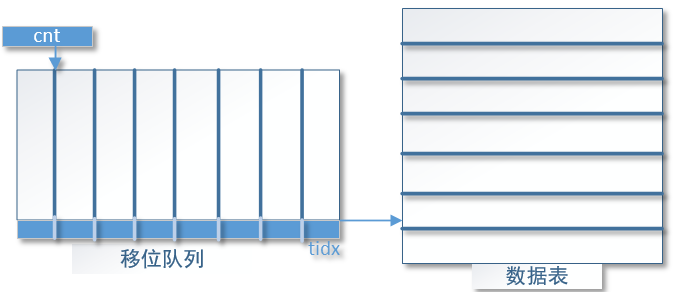
\includegraphics[width=0.7\linewidth]{opt_shift_queue}
	\bicaption{低功耗的优化,移位队列加数据表。}{shift queue plus data table, a optimization for saving energy.}
	\label{fig:opt_shift_q}
\end{figure}


整个中间层和后端就是用这两个最为基本的数据结构组合而成。一些复杂的操作流程,都可以规约为对队列的操作。以这样的角度去设计乱序多发射处理器,将会最大限度的控制复杂度,做到最大程度的简化。

\subsection{前端指令队列}\label{subsec:frontq}
除了有高速缓存的前端,高性能处理器在后端(包括中间层)中同样有一定数量的指令缓存,在BIAN的设计中被划分为了三个执行梯队(参见章节\ref{subsec:exe_hierarchy})。前端指令队列存储第三梯队的指令,入口位于inst back级,出口位于rename级。前端指令队列的结构如图\ref{fig:front_q},为循环队列的实现形式,所以第三梯队的指令是顺序被执行的。
\begin{figure}[!htbp]
	\centering
	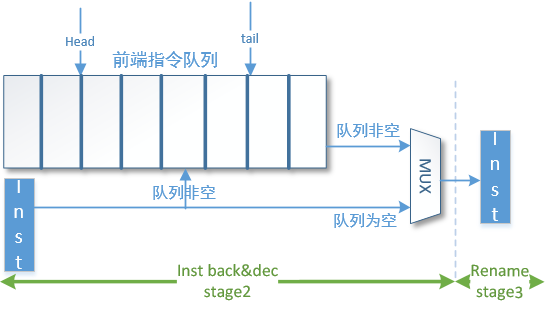
\includegraphics[width=0.7\linewidth]{front_inst_q}
	\bicaption{前端指令队列}{The queue storing for frontend instruction .}
	\label{fig:front_q}
\end{figure}

队列的每一项能够容纳两条指令,与取指器的宽度保持一致,让前端指令进入队列的逻辑保持简单。从取指单元取回来至少一条有效的指令,当后端没有剩余空间来接收时,会被压入该队列,从而不影响取指单元的继续取指。直到该队列满了,才会阻塞前端。BIAN中此队列有16项,容量一共是32条指令。执行benchmark程序时,几乎都为空的状态,主要用来隐藏16个周期的访存延迟。

\subsection{分支跳转预测队列}

从前端传来的不仅有指令,同时也有转移猜测的信息。直观上来讲,转移猜测的信息可以和指令一起存放在章节\ref{subsec:frontq}的前端队列中。但是由于前端指令队列的入口在inst back级,对于转移预测信息来说入队列的时机太早,所以不同于前端指令队列,分支的预测信息专门存放在分支预测队列中,在图\ref{fig:predict_q}流水线的中间部位。
\begin{figure}[!htbp]
	\centering
	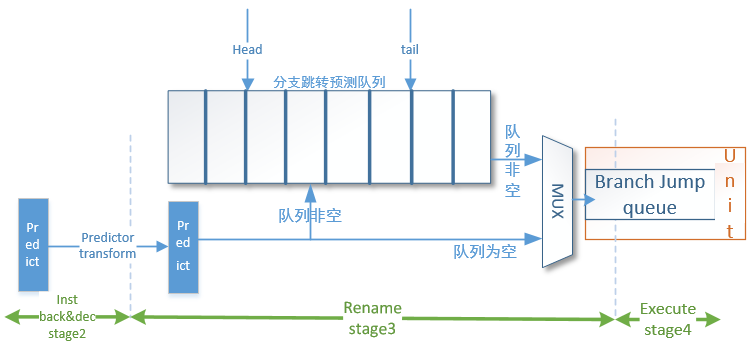
\includegraphics[width=0.8\linewidth]{branch_j_pipeline.png}
	\bicaption{分支跳转流水线}{The pipeline of branch jump instruction.}
	\label{fig:predict_q}
\end{figure}

该队列为循环队列,入口和出口均在rename级,所以预测信息可以等到rename级预测单元对预测信息做最后的修改再存入队列中。使用二选一的旁路来保证和出前端指令队列的指令是一一对应的。最后预测的信息会被写入分支跳转单元中的队列。因为前端在inst back级做了当两条并行指令同时为跳转指令将其串行化的逻辑,所以保证每一周期最多只有一条跳转指令。所以分支预测队列每一项的容量是一条指令的预测信息(通过二选一的逻辑选择出跳转指令的预测信息),这样,面积的开销减少一半。

\subsection{为什么不需要PC队列}

前端传来的不仅有指令和转移猜测信息,还有PC。直观来看,也应该有一个PC队列来存放每个指令所在的PC值。但是仔细一想,每一周期的PC其实也可以由分支预测队列存放的预测目标以及重定向使能信号推导出来。如果预测信息是错误的,也可以通过后端发送的取消信号重新更正PC。所以没有必要把pc存起来,这样,大大降低了处理器的面积开销。

\subsection{发射队列}

发射队列负责存储第二梯队的指令,结构如图\ref{fig:rename_inst_q},出口和入口都位于rename级,指令先进过重命名表,将逻辑寄存器号转换为物理寄存器号,并分配好资源后压入队列的尾部(为了做一个周期的优化,也做了旁路,当发射队列空时,不需要进入发射队列而可以直接选择发射)。不同于之前提到的各个队列,发射队列采用的是移位队列的实现方式(图\ref{fig:opt_shift_q}),这样可以支持乱序出队列,是实现乱序化最重要的一步。在细节上,移位队列每项的信息可以精简到两个物理寄存器号加上是否需要继续侦听的标志位和一个用来索引数据表的id号。这样,每项总共20-bit左右,其余的信息可以存储在数据表中,故移位逻辑的功耗得到了有效的控制。

由本章节开头对移位队列的分析,出队列项数为1是移位队列最合适的设置。但是双发射乱序要求发射项数为2,为了能够兼顾这矛盾的两点,采用的是两路并行的发射队列,事实上,图\ref{fig:rename_inst_q}中只给出了其中一路。每路每一周期都会从队列里弹出一项读寄存器堆然后发射到执行级。入队列也是严格按照物理的位置静态地每一路至多压入一项,处于时序的考虑不会采用动态分配的策略(也即如果第一路的队列满了,第二路队列未满,偶数PC的指令不会被动态压入第二路队列中)。这样的设定虽然会产生两路队列指令数量不平衡的情况,但是会由下游的执行队列来很大程度的缓解。
\begin{figure}[!htbp]
	\centering
	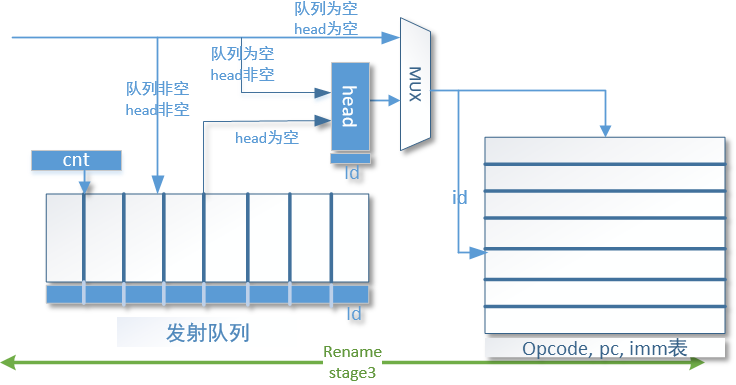
\includegraphics[width=0.8\linewidth]{rename_inst_q}
	\bicaption{单路发射队列}{One way of the inst issue queue}
	\label{fig:rename_inst_q}
\end{figure}

图\ref{fig:rename_inst_q}中的head是专门考虑电路时序的设计,这样发射的时候就不需要经过发射队列多选的过程。为了规整,移位队列主体为8项凑足2的幂次。若项数比8更多,侦听的电路效率就会下降。所以head的设计还增加了两条指令的容量。这样,两路发射队列总共的容量是18条指令。

在BIAN的发射队列设计中,有Alpha 21264,MIPS R10000和BOOM都没有的独特设计。从\ref{sec:meterial}的分析中看出,这三款处理器中,发射队列发射的指令必须是操作数都已经准备就绪的,当发射队列没有指令准备就绪时,这些处理器都没有打破僵局的机制和能力。但是BIAN处理器不同,发射队列依旧可以发射最早的指令,读取目前已经有效的操作数,然后发射到执行级,缓存入执行队列中(前提是执行队列未满),相当于是将指令的执行等级从第二级切换到了第一级。符合指令调度的直观。

\subsection{处理器状态控制单元}\label{subsec:state_unit}
在章节\ref{subsec:cpu_state}中,已经说明了什么是处理器的状态。处理器状态的正确变化是衡量处理器设计正确性的唯一标准,因此控制处理器状态变化的模块单元是处理器设计的重中之重。

无论是顺序处理器,超标量处理器,乱序处理器,本质上都是根据指令正确的改变处理器的状态。所以以一种更高的角度来看,高性能的处理器是能够高效的改变自身状态的机器(machine)。

乱序中最大的挑战在于处理器状态的维护和发生指令流发生错误的纠正。主要体现在三点上:
\begin{enumerate}[label=(\alph*)]
	\item 转移预测错误,要及时清除跳转指令后的错误指令流对处理器状态的改变,恢复至到跳转指令为止的处理器状态。
	\item 访存出现写后读冲突,但是后读的load指令先于写提交而且没来得及做数据前递,需要将状态恢复至到该load指令前面一条指令为止的处理器状态。前端重新从这条load指令起开始取指。这个在处理器设计的专业术语里叫做回滚。
	\item 例外和中断的发生。需要将状态恢复到中断例外指令之前的所有指令更新完的处理器状态。
\end{enumerate}

顺序执行的处理器,其状态是非常好维护的,因为指令都是顺序修改寄存器堆中寄存器值的,指令流出现错误也不会产生错误的处理器状态。但是乱序不一样,错误的指令流可以在未检测到之前对处理器状态做出改变。在目前的BIAN处理器设计中,实现的是RAM形式的重命名表,故处理器状态的恢复回溯也要以RAM重命名表为中心。下面是代码所描述的处理器状态的变量集合,以类的形式封装在一起。
\begin{scala}
	class State(val nEntry: Int) extends Bundle {
		val useing = UInt(nEntry.W)
		val usecnt = UInt(log2Ceil(nEntry+1).W)
		val maptb  = Vec(32, UInt(log2Ceil(nEntry).W))
		val rename = Vec(32, Bool())
	}
\end{scala}
	
基于RAM的重命名表在上述代码中是\texttt{maptb}变量,nEntry是物理寄存器堆的项数,所以$ log2Ceil(nEntry) $就是索引物理寄存器堆地址的位数。BIAN处理器设置了60项物理寄存器。其他变量的含义分别是:
\begin{enumerate}[label=(\alph*)]
	\item \texttt{useing}: 正在使用的物理寄存器分布向量,每一个物理寄存器占一位,1表示正在被使用,;0表示空闲,可以被分配。
	\item \texttt{usecnt}: 正在使用的物理寄存器计数器,产生分配物理寄存器的ready信号,比如需要分配一个物理寄存器需要条件usecnt < nEntry成立。
	\item \texttt{rename}: 逻辑寄存器号是否已经被映射到某一个物理寄存器号,如果是则为1,不是为0。含义是清晰的,用于写后写冲突中,后写的指令能够在指令提交时回收旧的物理寄存器。
\end{enumerate}

所以有了明确的状态刻画,需要有多少个\texttt{State}类只需要\texttt{new}出来即可。那么一共需要多少个\texttt{State}类呢?首先要有一个最新的状态,负责当前的重命名和物理寄存器号分配,这一个作为主要的\texttt{State}。其次为了精确的状态回溯,考虑要有状态的备份。回到上述提及的三种需要状态回溯的情况,可以分为两种不同的处理机制:第一种,发现指令流错误,马上撤销之后的指令流和处理器状态变化,发送重定向请求到前端;第二种,等到前面指令都已经顺序提交退出,再做发送重定向的请求,并撤销后续指令流和处理器状态变化。像转移预测错误因为比较频繁发生,所以一般做成第一种机制;而像回滚和中断例外,很罕见,可以做成第二种机制。BIAN处理器就是这么处理的。第二种机制需要有一个\texttt{State}备份记录至提交指令为止处理器的状态;第一种机制又可以有两种不同的做法,参见章节\ref{sec:meterial}中对Alpha 21264 (\ref{subsec:alpha})和MIPS R10000 (\ref{subsec:BOOM})的分析,在BIAN中采用的是MIPS R10000的做法,只针对每一条跳转指令做一个\texttt{State}备份。而在BIAN处理器中乱序部分最多支持四条分支跳转指令的投机,所以状态有四个备份用来回溯。代码如下:
\begin{scala}
	val latest = RegInit({ //当前用于重命名的最新的处理器映射状态
		val w = Wire(new State(nPhyAddr))
		w.maptb  := DontCare
		w.useing := 0.U
		w.usecnt := 0.U
		w.rename := VecInit(Seq.fill(32)(false.B))
		w
	})
	val commit = RegInit({ //是回滚和中断例外的状态备份
		val w = Wire(new State(nPhyAddr))
		w.maptb  := DontCare
		w.useing := 0.U
		w.usecnt := 0.U
		w.rename := VecInit(Seq.fill(32)(false.B))
		w
	})
	//nBrchjr = 4, 分别对应每一条投机执行的分支跳转指令的状态备份
	val backup = Reg(Vec(nBrchjr, new State(nPhyAddr)))
\end{scala}	

有了状态的描述,回溯恢复就是把相应要回溯的状态变量赋值给latest状态即可(省略复杂的细节),非常的简单直观。

除了基于重命名表的状态记录和回溯机制,作为处理器状态的主要控制单元,还有两大主要的功能:
\begin{enumerate}[label=(\alph*)]
	\item 指令id号的分配,载体是ROB,组织形式是循环队列,id号从尾指针顺序分配,从头指针顺序回收。
	\item 物理寄存号的分配。分配的时候在\texttt{latest}状态变量的\texttt{using}属性中,从左边找第一个1,从右边找第一个1,并行分配两个物理寄存器号。
\end{enumerate}

指令id号是标记处理器乱序部分顺序的唯一标识符。BIAN的分配的id号是5位的,对应于乱序部分最多可以in-flight 32条指令。

\subsection{分支跳转队列}

分支队列和访存队列就是面向后端的数据结构,分别在后面章节\ref{subsec:bj_unit}和\ref{subsec:ls_unit}中会详细说明设计中的亮点。

分支跳转队列的入口在中间层,说明是顺序分配资源进入队列,而不是不是执行时乱序分配的。原因很简单,因为分支跳转是控制相关的,带有顺序属性,在乱序中也要保持相对的顺序。采用的数据结构组织形式和发射队列类似,为移位队列,如图\ref{fig:bj_unit}。
\begin{figure}[!htbp]
	\centering
	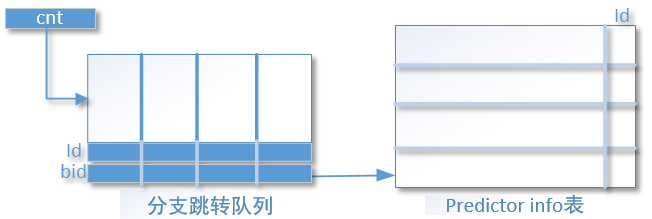
\includegraphics[width=0.8\linewidth]{branch_j_unit}
	\caption{分支跳转队列。}{The shift queue storing for branch and jump instruction.}
	\label{fig:bj_unit}
\end{figure}

\subsection{访存队列}\label{subsec:ls_queue}

解释两个和访存队列有关的问题:其一,直观来讲,访存指令并不是控制相关的,那么为什么访存单元队列的入口设置在中间层,要求顺序的时候分配资源呢?其二,从图\ref{fig:ls_unit}给出的访存队列数据组织结构中,为什么不和发射队列和分支队列一样采用的移位队列,而是用循环队列呢?

核心的原因在于:首先,对比普通寄存器数操作指令,写后写,写后读的冲突可以由重命名机制完美地解决,但是重命名机制却做不好访存指令的写后写,写后读冲突,因为访存的地址不是在rename级得到的,而是在乱序的执行级得到的。乱序执行是无法检测访存指令之间写后写,写后读的冲突。所以为了解决这个问题,这里就必须用队列的顺序分配来对保持访存指令之间的相对顺序。其次,因为store的写操作是对外的,所以已经超出了章节\ref{subsec:state_unit}中论述的处理器状态控制的范畴,要实现精确的状态恢复,store指令必须在LS commit级将数据顺序写回内存中,其顺序性需要有队列这样的first in first out的结构来保证。

队列类型不用移位队列而采用移位队列的原因在于:为了判读写后写,写后读的冲突,整个32位或者64位地址都将是关键信号,也要在移位队列中进行移位,如此一来功耗将会非常大。所以从功耗的开销和所获得的收益的角度来考虑,BIAN处理器做成6项循环LDQ和6项循环STQ,已经大概率的满足in-flight的32条指令中访存指令的存放需求。

\subsection{精确资源分配}
在中间层的设计过程当中,发现资源的精确分配逻辑非常复杂。资源的精确分配,指的是根据指令精确到对各个物理部件资源的不同需求和对应的各个物理部件单元剩余容量,做出资源分配。

这个逻辑的复杂性在于:
\begin{enumerate}[label=(\alph*)]
	\item 不同指令的需求是不一样的。有的指令有写寄存器的需求,所以需要分配物理寄存器;有的是跳转分支指令,在分支队列要分配项数;有的是访存指令,需要在访存队列中分配项数。
	\item 不同资源的剩余容量参差不齐,只要有一种资源指令有需求,但是无法分配,这条指令相关的其他指令都不能分配。
	\item 同一指令的需求是多样的,可能既需要物理寄存器,也需要访存队列
	\item 需要对两条并行的指令进行同时分配,第一条指令的分配情况会组合逻辑的作用于第二条指令发分配情况。所以并行的指令如果要实现精确分配物理资源就必须是串行的。
\end{enumerate}
\begin{table}[!htbp]
	\bicaption{中间层需分配资源列表。}{The list of resources in the Middle end.}
	\label{tab:resource}
	\centering
	\footnotesize% fontsize
	\setlength{\tabcolsep}{4pt}% column separation
	\renewcommand{\arraystretch}{1.2}%row space 
	\begin{tabular}{cc}
		\hline
		资源名称 & 备注 \\%inserts table 
		%\cline{2-9}% partial hline from column i to column j
		\hline
		指令标识符id   & 每条指令都必须分配,最多同时分配2项  \\
		物理寄存器号   & 有写寄存器的需求的指令分配,最多同时分配2项  \\
		发射队列entry & 每条指令都必须分配,每路队列最多分配1项  \\
		访存队列entry & 访存指令需要分配,最多分配2项 \\
		分支队列entry & 分支跳转指令除了jal类,最多分配2项 \\
		\hline
	\end{tabular}
\end{table}
\begin{figure}[!htbp]
	\centering
	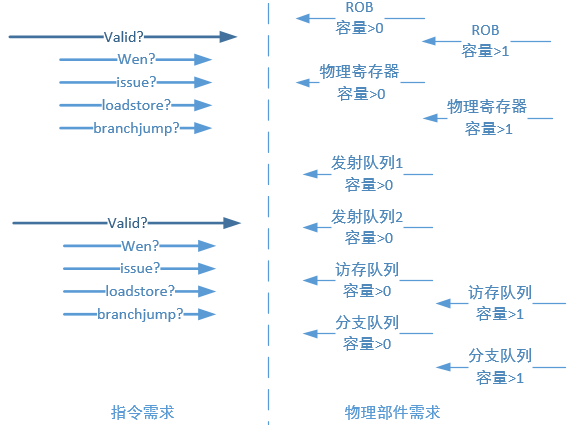
\includegraphics[width=0.7\linewidth]{issue_analysis.png}
	\bicaption{资源精确分配分析。}{analysis of precisely resources allocation.}
	\label{fig:issue_analysis}
\end{figure}

所以多发射宽度更高如四发射的很多处理器都采用了保守发射的逻辑来避免精确带来的复杂性。只要指令有效,就认为指令有所有的需求。换言之,在分配资源时只需要顾及指令是否有效即可。另外,在复杂处理器的设计中,由于各个部件单元的面积都很大,布局布线后的位置也会相隔较远,所以若采用精确发射走线延迟会很大。但是BIAN处理器后端面积不大,资源队列的项数较小,故走线延迟在可接受范围以内。另一方面,项数少就要采用精确分配的逻辑来节约使用。所以权衡之下,BIAN处理器中间层资源分配采用精确的方式,来提高资源的利用率和执行的效率。


BIAN处理器中间层需要分配的资源有五个,如表\ref{tab:resource}所示。
一方面是两条并行指令的各个需求以及是否有效,另外一方面是各个物理部件的容量信息,如图\ref{fig:issue_analysis}所示。

\section{后端的设计}
执行队列是完全属于后端的单元;分支跳转单元和访存单元除了队列入口在中间层外,部件的主体在后端。
\subsection{执行队列}\label{subsec:execute_q}

这个队列就是上文提及的执行等级的第一梯队,组织的格式同样是图9的移位队列,而且移位队列中entry的内容和发射队列保持一致,物理上就可以保证指令的相对顺序。缺点很明显 --- 面积开销很大,但是优点同样明显,执行快而且不需要读寄存器堆,将物理寄存器堆的读端口维持在4个,物理布局布线能够接受的水平。执行队列还有一个很重要的功能是及时平衡发射队列的指令数量。因为两个发射队列是独立平行的,每个队列只分别负责接收从前端送来的两条指令的有效的第一条和第二条。由于并不是每个周期的两个指令都是有效的,所以会导致发射队列指令数不平衡,影响到资源的利用率。依靠执行队列,当执行级两条指令同时因为操作数没有准备号被阻塞住时,接受来自含指令条数多的发射队列的那一条指令,从而起到平衡发射队列的作用。
\subsection{分支跳转部件}\label{subsec:bj_unit}
主体是分支跳转队列,对接着前端的转移预测器,构成了整个反馈回路的分支跳转系统。这一系统在高性能处理器的重要性仅次于访存系统。高性能的分支跳转系统在设计的时候有3大指标需要考虑:
\begin{enumerate}
	\item 高准确率  是设计的首要指标,90\%的准确率下处理器的IPC和95\%的准确率下的IPC都要相差很多。
	\item 低周期数  同样是设计中要考虑的重要指标。反馈周期的定义是从投机的取跳转指令的下一周期的指令开始,到跳转指令被执行能够发出重定向信号为止,一共需要经过的周期数。
	\item 低延迟,小面积,低功耗。
\end{enumerate}
而在分支队列的设计中,主要对应的指标就是低周期数。分支队列的结构如图13所示,目前的设计中有4项,也就是说乱序的32条指令中允许有4条分支,这四条分支能够把整个指令流分成5段,所以每段的平均长度在$6\sim7$之间,恰好也符合跳转分支指令在总指令中的平均占比。回到图13,会发现和图9的标准移位队列有些出入。主要体现在的地方是分支队列和分支信息表都多了id域(bid是需要的,因为要索引数据表)。移位队列要有id域是由于中间层就要分配,但是后端的执行是乱序的,执行完成回到分支队列就要用到cam查找去匹配到属于自己的那一项entry,然后再靠对应的bid来索引table得到相应的信息。理论上还存在着另外一种方案,就是ram查找,如果用ram,就必须在每一条指令都带上bid,比cam逻辑麻烦,而且分支跳转队列只有4项,算得上项数很少了。

table中的id域的作用同样是为了cam查找。这个id域是可以不要的,因为可以先通过cam索引移位队列得到对应的bid然后再去索引table。但是如果加上id域,就意味着两个结构的查找可以做到并行。这并行的考虑正是为了降低反馈周期数而专门设计的。反馈做到可以走组合逻辑路线的就不走时序逻辑路线。什么情况下可以用组合逻辑而又不影响CPU整体的延迟。仔细分析一下,除了jr类指令需要读取寄存器来进行运算,其他的分支跳转指令都是直接通过pc和指令中的立即数域进行符号拓展就可以得到跳转地址的,所以到中间层的时候跳转地址就能够被计算出来,顺势就可以存入分支表中。而且还需要注意的是像j类指令直接知道跳转地址和一定要跳的指令,是不会进入分支队列的,在risc-v中只有branch和jr两类指令会进入队列。在执行级,branch真正做的操作只有两个操作数的比较,工作量相对较少,所以就非常适合组合逻辑直接反馈;而jr类指令因为要算地址,所以先进入队列和表项中,然后在下一周期再对前端做出反馈。
\subsection{访存部件}\label{subsec:ls_unit}
%阐述对load/store指令的特殊优化
访存部件的主体是3个循环队列组成,分别是LDQ,STQ和load/store队列,在重命名阶段分配,每个队列的每项都带有全局id,后端的每个流水级利用cam查找到队列中对应的项并做出更新。LDQ和STQ意义和功能都非常明确,资源的释放也都是在load和store指令commit的时候。但是被称为load/store队列的这第三个队列又有什么设计上的考虑和用意。

引入这第三个队列的考虑在于:凡是在中间层分配的队列资源,都有一个缺点,就是只要存在指令有入队列的请求,但是队列已满,那么后端就会一律暂停接收来自前端或者中间层前端指令队列的指令。所以跳转指令和访存指令都存在这个问题。对于跳转指令而言,由于是控制相关的,维护起来代价巨大,不易做多,不得不牺牲这方面的考量。而访存指令的情况又不同于跳转指令,首先是一长串的连续的访存指令不少见,尤其在访存密集的程序中,6项的LDQ或者6项的STQ如果遇到这种情况不够用,就必须阻塞后面的指令。但此时有可能发射队列还很空,例如也就6条load指令分散于两个之中,也就是每个队列3条,乱序资源得不到有效的利用,所以有必要对LDQ和STQ扩容;但是另外一方面,在一长串的访存类指令中,一般都是处于同一或者相邻cache行的,所以真正需要长时间在执行中的访存指令也相对较少,不宜对LDQ和STQ扩容,增加无谓的面积去存储肯定暂时得不到的地址数据。

综上所述,现在面临的两难局面是:一边为了提高乱序资源利用率而主张扩容,一边为了不增加访存队列面积而反对扩容。解决的方案就是增加一个load/store队列。这个队列里每一项的信息非常少,只有一个id,一个访存类型,一个load/store标记位。这个队列做到8项,占用的总资源也不会超过80bits,非常的小巧。这第三个队列和STQ和LDQ的交互大致是如图14所示,load/store指令会优先选择进入STQ或者LDQ,只有到LDQ或者STQ满了,才会填入load/store队列。而STQ或LDQ释放的资源后也会优先分配给load/store队列中的项,如果queue是空的,才会直接填入从中间层送来的访存指令信息。同时为了逻辑的正确性,必须规定凡是在这个loads/tore队列里的指令不能够被发射执行,直到该条访存指令被转移到了LDQ或者STQ,才能重新获得被发射的权利。load/store队列加上这个规定,将会提高处理器在运行访存密集程序上的性能。

访存部件涉及到后端所有的流水级,而且又是与CPU的外部信号交互,是后端中最复杂的一个部件。列举每一级的操作:
\begin{enumerate} %TODO: change to table
	\item rename级 --- 访存指令进入相应的队列
	\item exe级 --- 计算出访存的地址写入相应的队列中
	\item LS memory级 --- 向外发出load请求,并且遍历队列得到写后读的相关forward信号
	\item data back\&fwd级 --- 数据load回来,进行必要的forward操作,练到写回总线
	\item LS retire级 --- 如果是load指令直接退出;如果是store指令往memory写完数据之后退出,同时store要做相关的backward操作,判读是否与已经取指回来的load指令有写后读的冲突,以便作必要的回滚。
\end{enumerate}
上述只是粗略的说明,并不准确,也省略了很多细节。由于写后读的冲突的存在,使得STQ和LDQ虽然是两个队列但有着密切的关联。维护这种联系的被我叫做forward和backward的两种操作。forward操作的主体是正要访存的load指令,动作是在STQ中前向扫描在该load指令之前的store指令,如果有地址冲突,store的数据就要前递到load的数据域中。backward的操作主体是处在STQ队列头部的store指令,动作是在LDQ中后向扫描在该store指令之后的load指令,如果存在读写地址冲突的情况,并且对应的load指令并没有来得及完成forward操作,就要向CPU状态总控单元发出回滚的请求。如下图所示:
\begin{figure}[!htbp]
	\centering
	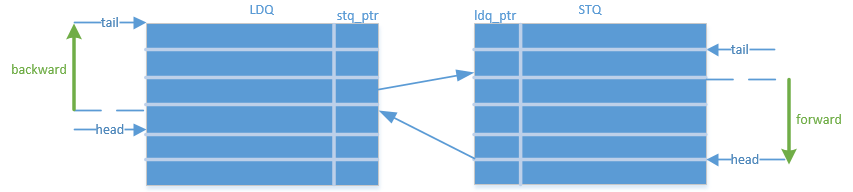
\includegraphics[width=\linewidth]{fwdbwd}
	\caption{forward \& backward示意图}
\end{figure}

为了确定forward和backward的起点,在原来的队列中各要加入指针域,在LDQ中是索引STQ的指针stq\_ptr,在STQ中是索引LDQ的指针ldq\_ptr。
\subsection{特权态指令执行的初步方案}
前面提到的后端各个数据结构大多都是针对用户态指令的,而特权态指令相对稀少而且特殊,目前还没有来得及针对risc-v好好分析一下特权态指令的依赖关系来进行优化,初步的方案是特权指令一律不会进入发射队列乱序化,而且一定要等到ROB为空时才能够直接发射执行。
\subsection{后端状态回溯机制}
状态的回溯在前面中间层的CPU状态控制单元已经有所提及,除了CPU状态控制单元负责CPU状态的回溯以外,对于后端其他数据结构的状态回溯因为有一个很好的抽象也就显得非常的简单直观。这是因为后端和中间层都是由队列构成的,或者是移位队列或者是循环队列。对于移位队列,如果是例外中断或者访存回滚,计数器置为0即可;如果是跳转指令取缔,将计数器置为id号小于该跳转指令的指令个数。对于循环队列,同理操纵head和tail指针即可。
\section{总结}
前端的章节中已经提到取指器的时序非常好,所有从后端传递的反馈信号都是锁一拍才会对取指器产生作用。而BTB也对其数据结构做了相应的物理的优化。前端是3级的流水,指令在第3级产生,被送到连接前后端的中间层,中间层先经过重命名把逻辑寄存器地址转化为物理寄存器地址,紧接着去索引物理寄存器堆读取数据出来直接送到锁存器,或者其实物理寄存器可以做成一个同步ram。CPU的最长路径极有可能会是这一条,目测估计要经过34级们左右。与这条路径并行的是物理资源的分配以及精确发射。如果发射队列为空就直接可以进入执行级执行,否则先进入发射队列轮循侦结果总线和旁路总线的信号。结果总线顾名思义就是结果已经得到的写回信息,而旁路总线指的是当前正要被发射,正在重命名读寄存器送到exe级执行的信号,换言之是预言下一拍就会得到结果的前递信号。由于commit总线的宽度是4,regfile的的写端口是4个,所以两类前递总线各有4组,总共8组。前递逻辑是时序也是比较紧张的,目测和中间层逻辑门级数要少一两级,但是相差不大。执行级依据内部微码对操作数进行运算,当然被送到exe级存在操作数还没有准备好的情况,将其压入执行队列。但是执行队列限定每一次只允许一条指令入队。处于平衡队列的考虑,如果同时出现两个发射队列的头部都没有准备好操作数,优先选择指令条数多的队列的头部指令入队。对于跳转指令和访存指令这种特定类别的指令执行控制,参考。%TODO
